% \handouts
% \ifx\handouts\undefined
\documentclass[10pt,dvipsnames,t,handout% (Un)comment ",handout" when (not) doing handouts
,aspectratio=169% Comment out if you want 4 by 3 (default)
]{beamer}% \else
%\documentclass[xcolor=svgnames,handout]{beamer}
%\fi

\mode<presentation>
{
  \useoutertheme{miniframes}
  \setbeamercovered{transparent}
}

\setbeamertemplate{footline}[frame number]

\setbeamertemplate{blocks}[rounded][shadow=true]

%\usecolortheme{seahorse}
\usecolortheme{rose}
%\usepackage{pictex}

\usepackage{babel}
\usepackage[utf8]{inputenc}
\usepackage{times}
\usepackage[T1]{fontenc}
\usepackage{moreverb}
\newcommand{\code}[1]{\texttt{#1}}
\newcommand{\sini}[1]{\textcolor{Blue}{#1}}

\newcommand{\E}{\mathrm{E}}
\let\overbatim\verbatim
\let\endoverbatim\endverbatim
\newenvironment{vcode}%
{\bgroup\baselineskip=0.8\baselineskip\overbatim}%
{\endoverbatim\egroup}

\newcommand{\indep}{\perp\!\!\!\!\perp}


\newcounter{demo}
\newcommand{\Demo}{\stepcounter{demo}\frametitle{Demo \arabic{demo}}}

\title{Introduction to causal inference} 

\author{Krista~Fischer}

\institute[TY] % (optional, but mostly needed)
{
  Institute of Mathematics and Statistics, University of Tartu \\
    Institute of Genomics, University of Tartu \\
   Estonian Academy of Sciences
}

\date[Tartu 2019] % (optional)
{Statistical Practice in Epidemiology, Tartu 2023}


\begin{document}

\begin{frame}
  \titlepage
\end{frame}

\section*{Outline}
\begin{frame}
\tableofcontents
\end{frame}

\section{How to define a causal effect?}

\begin{frame}
  \frametitle{Statistical associations vs causal effects in epidemiology}
  \begin{block}{}
  Does the exposure (smoking level, obesity, etc) have a \alert<2>{causal effect} on the outcome (blood pressure, cancer diagnosis, mortality, etc)?
  \end{block}
is not the same question as   
 \begin{block}{}
  Is the exposure \alert<3>{associated} with the outcome?
  \end{block}
 Conventional statistical analysis will answer the second one, but not necessarily the first. 
%  \end{itemize}
\end{frame}

\begin{frame}
	\frametitle{Example}
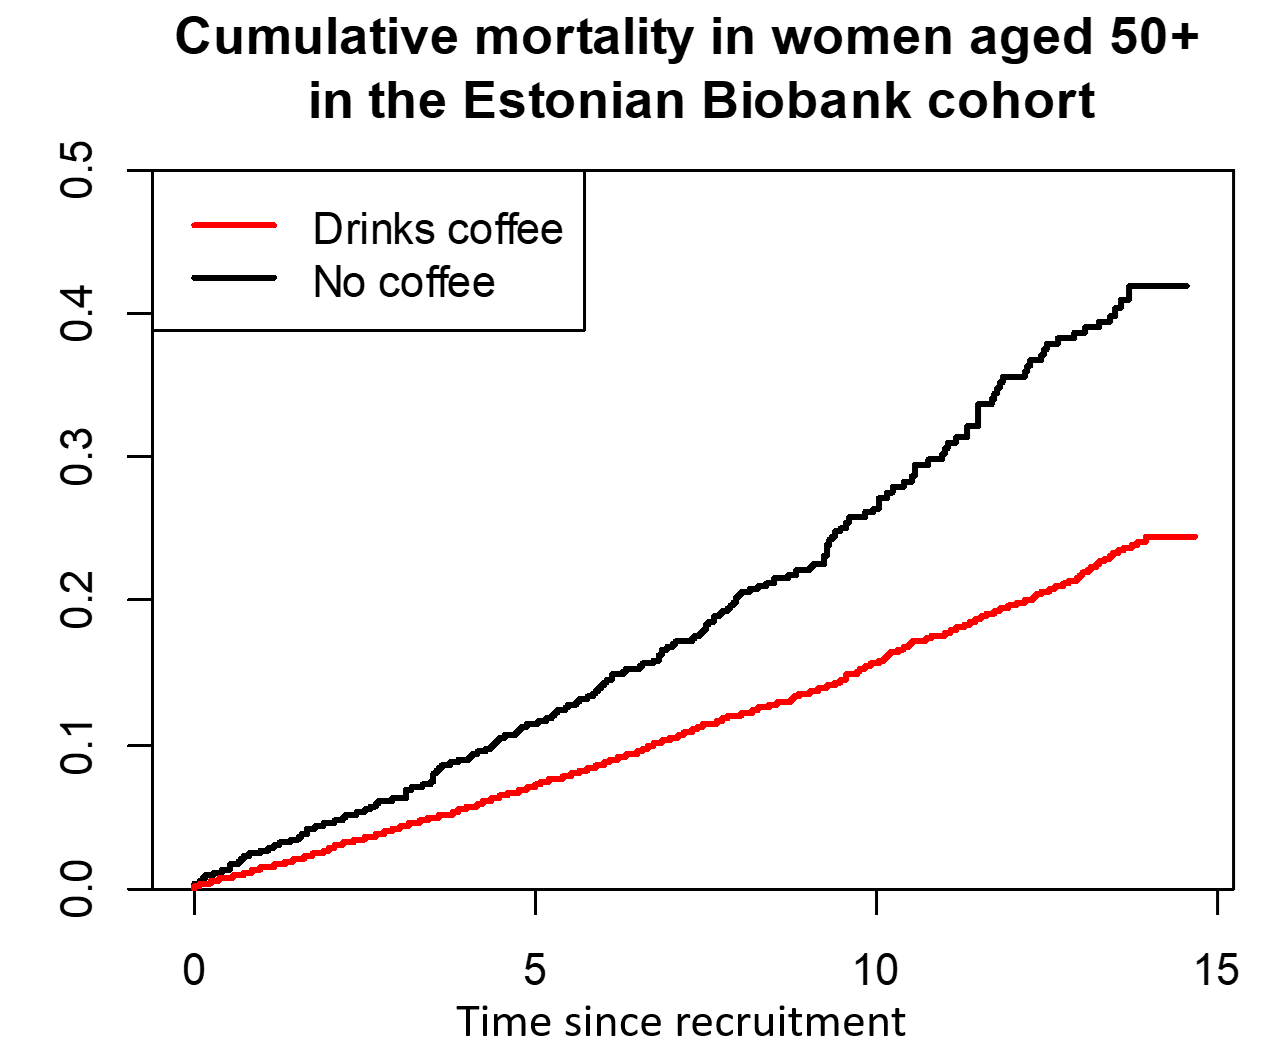
\includegraphics[width=6cm]{kohv_egv_1} \\
\begin{block}{}
Does coffee-drinking prolong life? \\
(so drastically???)
\end{block}
\end{frame}

\begin{frame}
	\frametitle{Example (cont.)}
	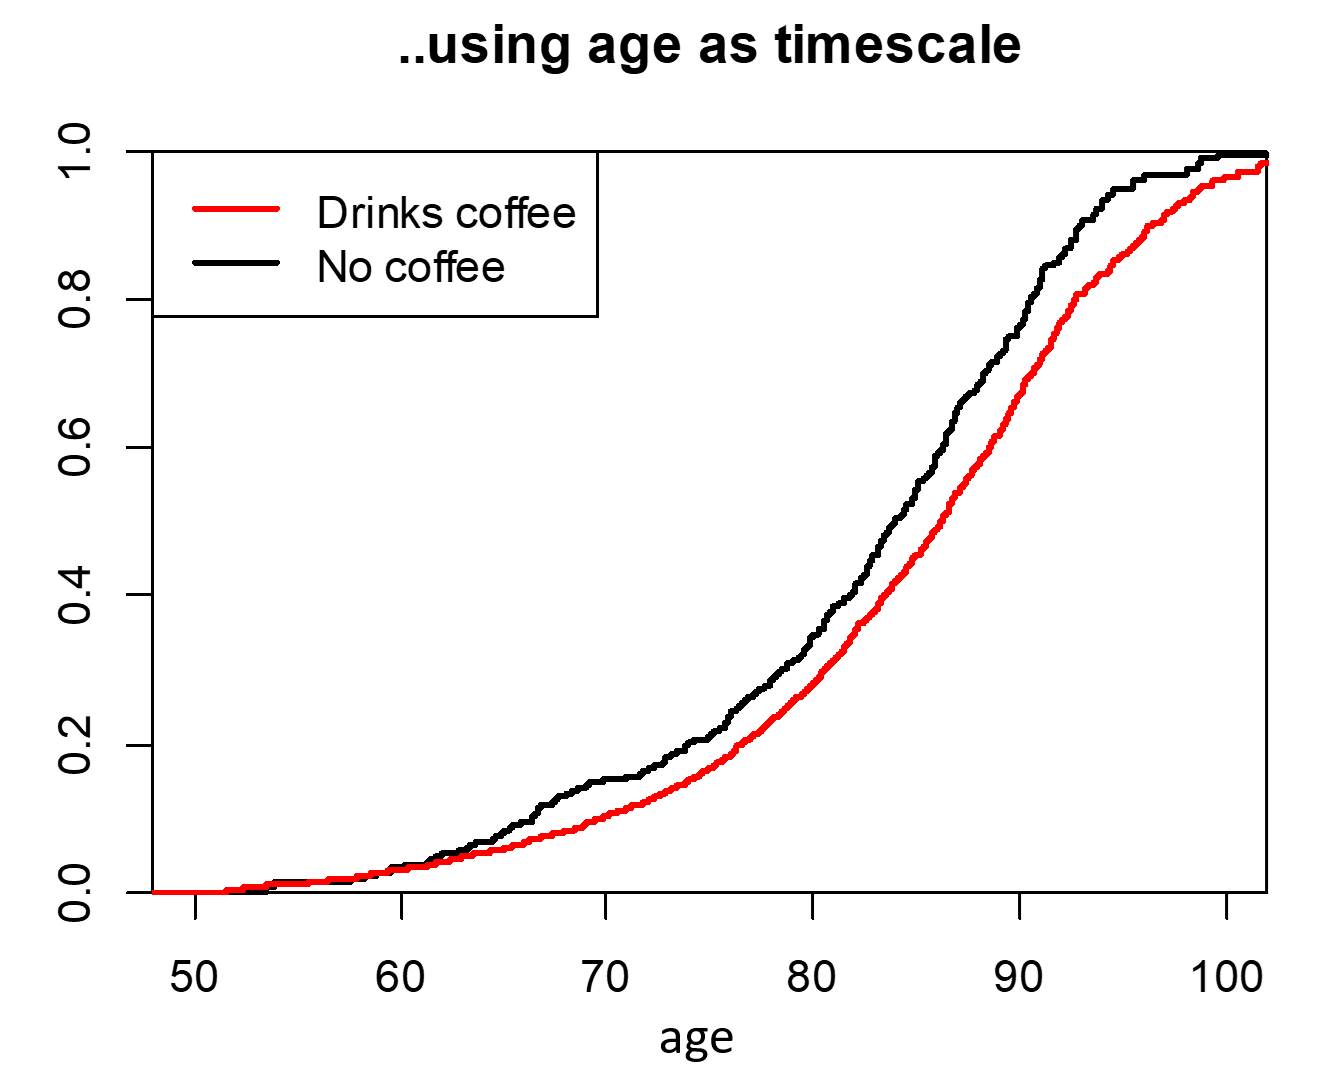
\includegraphics[width=6cm]{kohv_egv_2} \\
\begin{block}{}
	Does coffee-drinking prolong life? \\
Or: \textcolor{blue}{do coffee-drinkers live longer (for several reasons)?}
\end{block}
\end{frame}


\begin{frame}
	\frametitle{How to define causal effects (properly)?}
	\begin{itemize}
		\item One can think of some basic guidelines (sometimes called as ``criteria'') that must be satisfied for causal effect to be identifiable. 
		\item Such principles may include temporality (cause preceding the outcome), consistency (reproducibility), monotonicity (dose-response), plausibility (e.g. biologically), etc. (Bradford Hill's guidelines)
		\item \alert{However, although such general guidelines are useful, they are often not sufficient to establish causality}
	\end{itemize}
\end{frame}

\begin{frame}
\frametitle{Causal effects and counterfactuals}
\begin{itemize}
\item To define causal effects more properly, \alert<1>{counterfactual} (what-if) thinking is useful.
\item Mathematically, the individual causal effect can be defined as the difference 
 \[Y^1 - Y^0,\]
where $Y^1=Y(X=1)$ and $Y^0=Y(X=0)$ are defined as individual's \alert<2>{potential (counterfactual)} outcomes if this individual's exposure level $X$ were \alert<2>{set} to 1 or 0, respectively. 
\item Example: $Y^1$ individual's blood pressure, if he/she were a smoker; $Y^0$ individual's blood pressure, if he/she were a nonsmoker;
\item For a particular individual, either $Y^1$ or $Y^0$ can be observed at any moment. 
%\item Sometimes people (e.g J. Pearl) use the \alert<3>{``do''} notation to distinguish counterfactual variables from the observed ones: $Y(do(X=1))$ and $Y(do(X=0))$.     
\end{itemize}
\end{frame}


\begin{frame}
	\frametitle{The ``na\"ive'' association analysis}
	{\small  \begin{itemize}
			\item With a binary exposure $X$, compare average outcomes in exposed and unexposed populations:
			\[E(Y|X=1) - E(Y|X=0)\]
			\textcolor{blue}{Is cancer incidence different in smokers and nonsmokers?}
			\item But mostly:
			\[E(Y|X=1) \ne E(Y^1)\]
			\textcolor{blue}{Cancer risk in smokers is not the same as the potential cancer risk in the population if everyone were smoking}
			\item Similarly:
			\[E(Y|X=0) \ne E(Y^0)\]
			% \textit{Cancer risk in nonsmokers is not the same as the potential cancer risk in the population if there were no %smokers}
			\item In most cases there is always some \alert{unobserved confounding} present and therefore the
			na\"ive analysis does not provide causal effect estimates.  
	\end{itemize}}
\end{frame}



\begin{frame}
	\frametitle{Potential outcomes (counterfactuals) in different settings}
	\begin{itemize}
		\item \alert<1>{Randomized trials}: probably the easiest setting to imagine $Y(X)$ for different $X$
		\item \alert<2>{``Actionable'' exposures}: smoking level, vegetable consumption, \ldots -- potential interventions may alter exposure levels in future.
		\item \alert<3>{Non-actionable exposures}: e.g genotypes. It is difficult to ask \emph{``What if I had different genes?''}. Still useful concept to formalize genetic effects (heritability, attributable risk).
		\item \alert<4>{Combinations}: With X-- a behavioral intervention level, Z--smoking level and Y--a disease outcome, one could formalize the effect of intervention on outcome by using $Y^{X, Z(X)}$
	\end{itemize}
\end{frame}

\begin{frame}
	\frametitle{A causal model in terms of potential outcomes}
	\begin{itemize}
		\item More generally $Y^x$ is defined as the potential outcome following the exposure level $X=x$
		\item A \alert{linear causal model} can be specified as 
		\[Y^x_i -  Y^0_i=  x \beta_1 + \varepsilon_i, \ \; \mbox{ with } E(\varepsilon_i|x)=0\]
		\item Note that the observed outcome $Y_i = Y_i^{x}$ for individuals with $X_i=x$.   
		\item The model could be generalized to include nonlinear terms or interactions with other covariates, or as a generalized linear model (logistic regression, survival model). 
		\item However, as we don't observe $Y^0$ and $Y^x$ (with $x>0$) for the same individuals at the same time, thus it is not straightforward to actually fit the model on data.  
	\end{itemize}
\end{frame}

\begin{frame}
	\frametitle{Statistical model vs causal model}
	\begin{itemize}
        \item More generally $Y^x$ is defined as the potential outcome following the exposure level $X=x$
		\item A \alert{linear causal model} can be specified as 
		\[Y^x_i -  Y^0_i=  x \beta_1 + \varepsilon_i, \ \; \mbox{ with } E(\varepsilon_i|x)=0\]
		\item Note that the observed outcome $Y_i = Y_i^{x}$ for individuals with $X_i=x$.   
		\item  	A \alert{classical linear regression} model: 
		\[Y_i = \beta_0 + X_i \beta_1 + \varepsilon_i, \ \; \mbox{ with } E(\varepsilon_i|X_i)=0\]
		or 
		\[E(Y_i|X_i) = \beta_0 + X_i \beta_1. \]
		\item 
		\alert{ When are the two equivalent?}
	   
	\end{itemize}
\end{frame}


\begin{frame}
	\frametitle{Statistical model vs causal model}
	\begin{itemize}
		\item Rewrite the linear causal model as 
		\[Y^x_i =  Y^0_i +  x \beta_1 + \varepsilon_i, \ \; \mbox{ with } E(\varepsilon_i|x)=0\]
		\item Note that this would be equivalent with the classical linear model, if 
		 $$E(Y^0_i + \varepsilon_i|X_i)= \beta_0,$$ 
		 \alert{thus when the potential exposure-free outcome $Y^0$ is not associated with the exposure $X$}
		\item  For instance, this would mean that in the absence of smoking, the cancer risk for current smokers and current nonsmokers would be the same ($E(Y|X=0) = E(Y^0)$).
		\item In other words, the two models are equivalent in the absence of \alert{confounding}. 	
	\end{itemize}
\end{frame}



\begin{frame}
 \frametitle{Classical/generalized regression estimates vs  causal effects?}
 \begin{itemize}
 \item In the presence of confounding, regression analysis provides a biased estimate for the true causal effect
\item To reduce such bias, one needs to collect data on most important confounders and adjust for them
\item However, too much adjustment may actually introduce more biases   
\item Causal graphs (Directed Acyclic Graphs, DAGs) may be extremly helpful in identifying the optimal set of adjustment variables
\end{itemize}
 \end{frame}

\begin{frame}
	\frametitle{DAGs: directed acyclic graphs}
	\begin{itemize}
		\item A Directed Acyclic Graph (DAG) is a graphical representation of the causal association structure in the data, where variables are presented as nodes (points) and the associations are presented as edges (lines, arrows);
		\item Thus an arrow pointing from variable $X$ to a variable $Y$ on such graph represents a causal effect of $X$ on $Y$.
	\end{itemize}
\begin{center} 
{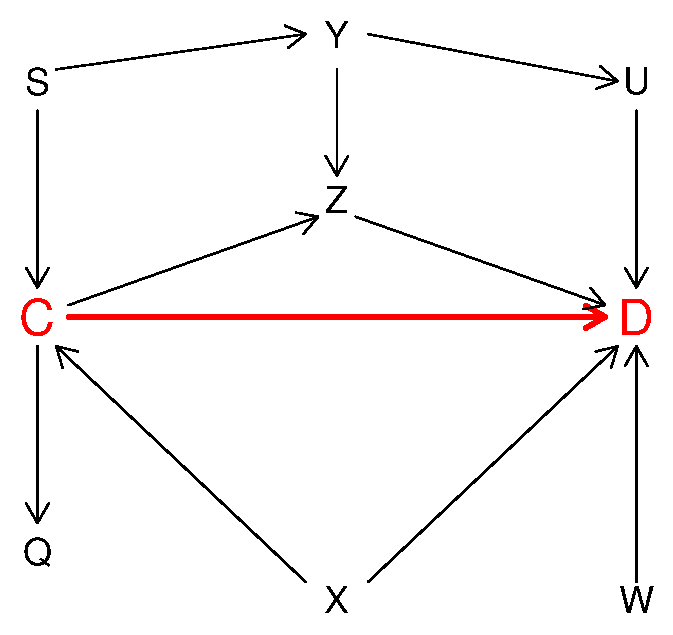
\includegraphics[width=0.3\textwidth]{keeruline2}}\\
\end{center} 
\end{frame}


\section{Causal graphs, confounding and adjustment}


\begin{frame}
	\frametitle{``Classical'' confounding}
	Third factors  Z influence both, X and Y \\
	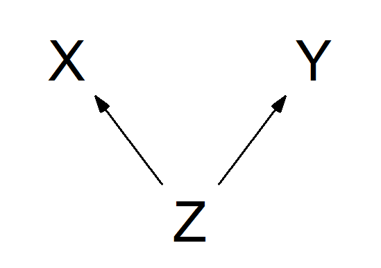
\includegraphics[width=4cm]{conf1}\\
	Also called as \alert{backdoor path} between $X$ and $Y$. \\
	
\noindent {\small Implied statistical associations ($Y$ is not independent of $X$ in general, but it is independent of $X$, conditional on $Z$):}
$$X \not\indep Y \; \hspace{0.5cm}  X \indep Y|Z$$
\noindent {\small 
	$X$ and $Y$ are independent, conditional on $Z$, but marginally dependent.}
	
\end{frame}

\begin{frame}
	\frametitle{``Classical'' confounding, mathematically}
\begin{columns}
\begin{column}{5cm}
\mbox{ } \\
	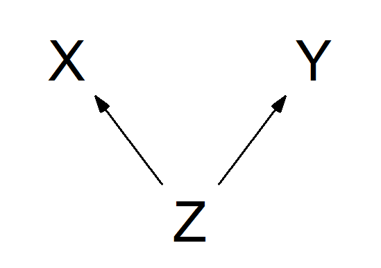
\includegraphics[width=4cm]{conf1}
	\mbox{}\\[0.5cm]
Assume:
$$X= b_{0x} + b_{zx}Z + \varepsilon_x, \ \E(\varepsilon_x|Z)=0 $$  
$$ Y= b_{0y} + b_{zy}Z + \varepsilon_y, \ \E(\varepsilon_y|Z, X)=0. $$
\end{column}
\begin{column}{7cm}
Now: 
$\E(Y|X) = b_{0y} + b_{zy}\E(Z|X). $ \\[0.2cm]
If  $b_{zx} \ne 0$, then also  $r_{zx} \ne 0$ and so 
$$ \E(Z|X) =  b_{0z}+ b_{xz}X, \mbox{ where }b_{xz} \ne 0$$. 
We see that:
$$\E(Y|X) = b_{0y}^* + b_{xz}b_{zy}X. $$

\begin{block}{}\alert{One should adjust the analysis for $Z$, by fitting a regression model for $Y$ with covariates
	$X$  and $Z$.} 
There is a causal effect between $X$ and $Y$, if the effect of $X$ is present in such model. \end{block}
\end{column}
\end{columns}
\end{frame}


\begin{frame}
	\frametitle{Example: COVID vaccination and Simpson's paradox}
\begin{block}{Suppose there are COVID infections in:}
\begin{itemize}
\item 3000 unvaccinated individuals, 90 needing hospitalizations
\item 1000 vaccinated individuals, 30 needing hospitalizations
\end{itemize}
\alert{No effect of vaccination?} 
\end{block} 
\pause 
	More detailed data: \\[0.2cm]
\begin{tabular}{|c|c|c|c|c|}
	\hline 
	age & vaccination & total & hospitalized & \% hospitalized \\
	\hline  
	$\ge 60$  & no & 100 & 24 & 24\% \\
	& yes & 300 & 24 & 8\% \\
	\hline 
	$<60$  & no & 2900 & 66 & 2.3\% \\
	& yes & 700 & 6 & 0.9\% \\
	\hline 
	all ages & no & 3000 & 90 & 3\% \\
	& yes & 1000 & 30 & 3\% \\
	\hline 	
\end{tabular}
\mbox{}\\[0.2cm]

%	\begin{block}{}
	\alert{Age is a confounder here!}

\end{frame}

\begin{frame}
	\frametitle{COVID vaccination and Simpson's paradox}
	Real data from Estonia (August 2021): \\[0.2cm]
	\begin{tabular}{|c|c|c|c|c|}
		\hline 
		age & vaccination & total & hospitalized & \% hospitalized \\
		\hline  
	$\ge 60$  & no & 186 & 50 & 26.9\% \\
          & yes & 202 & 16 & 7.9\% \\
	\hline 
	$<60$  & no & 3075 & 57 & 1.9\% \\
	       & yes & 666 & 5 & 0.8\% \\
	\hline 
    all ages & no & 3261 & 107 & 3.3\% \\
               & yes & 868 & 21 & 2.4\% \\
\hline 	
\end{tabular}
\mbox{}\\
\end{frame}


\begin{frame}
	\frametitle{Causal chain (mediation, front-door path):}
	The effect of X on Y is \alert{mediated} by  Z:   \\[0.5cm]
	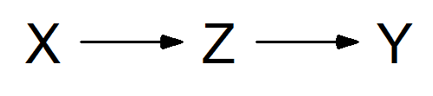
\includegraphics[width=4cm]{chain}\\[0.5cm]
	
	$Y = \beta_0 +  \beta_{xy} X + \beta_{zy} Z + \varepsilon $, \\[0.3cm]
	
	\pause
	\begin{itemize}
		\item 
	\alert{Don't adjust for $Z$},  if you are interested in the \alert{total effect} of $X$ on $Y$  
\item \alert{Do adjust for $Z$},  if you are interested in the \alert{direct effect} of $X$ on $Y$ 
\item Adjusted analysis is valid only when the $Z$-$Y$ association is unconfounded! 
\end{itemize}
	

\end{frame}

\begin{frame}
\frametitle{The case of a \alert{collider}: adjustment is sometimes wrong!}
X and Y have an effect on  Z:   \\[0.5cm]
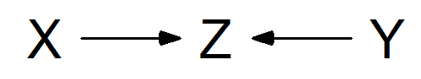
\includegraphics[width=4cm]{collider}\\[0.3cm]

$Z = \beta_0 +  \beta_{xz} X + \beta_{yz} Y + \varepsilon,$ with $\beta_{xz}\ne 0$ and $\beta_{yz}\ne 0$ \\[0.2cm]
hence, there exist parameters 
$\beta_{xy}\ne 0$ and $\beta_{zy}\ne 0$, so that: \\
$Y = \beta^*_0 +  \beta_{xy} X + \beta_{zy} Z + \varepsilon^*. $\\[0.2cm]
$$X \indep Y \; \hspace{0.5cm} 
X \not\indep Y|Z$$

 
\pause
\begin{block}{ }
We see the association between $X$ and $Y$ only when the ``effect'' of  $Z$ has been taken into account. \\
\alert{But this is NOT a causal effect of $X$ on $Y$.} 
\end{block}

\alert<2>{One should NOT adjust the analysis for $Z$!}
\end{frame}

\begin{frame}
	\frametitle{\alert{Selection bias:} a special (but common) case of collider bias}
\begin{itemize}
	\item All analysis are done conditional on the selected sample
	\item However, selection itself might be a collider (Griffith et al. 2020, \href{https://www.nature.com/articles/s41467-020-19478-2
	}{https://www.nature.com/articles/s41467-020-19478-2
} ) \\[0.3cm]
\end{itemize}	

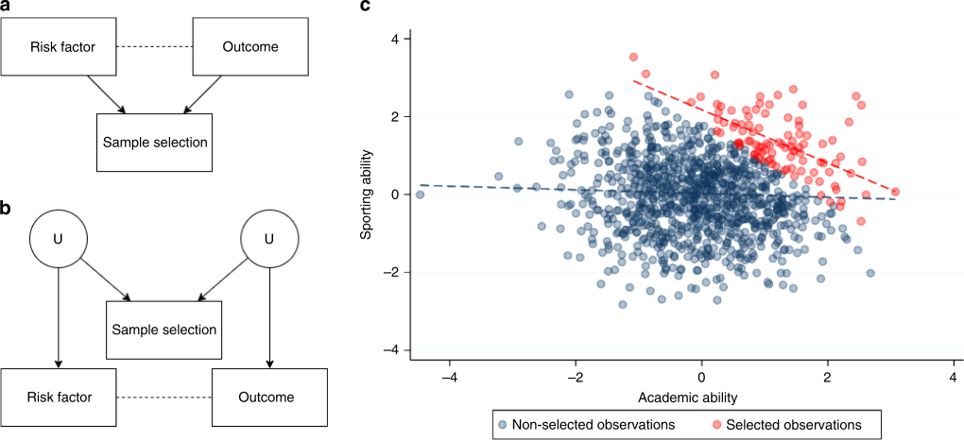
\includegraphics[width=11cm]{us_univ}

\end{frame}

\begin{frame}
	
	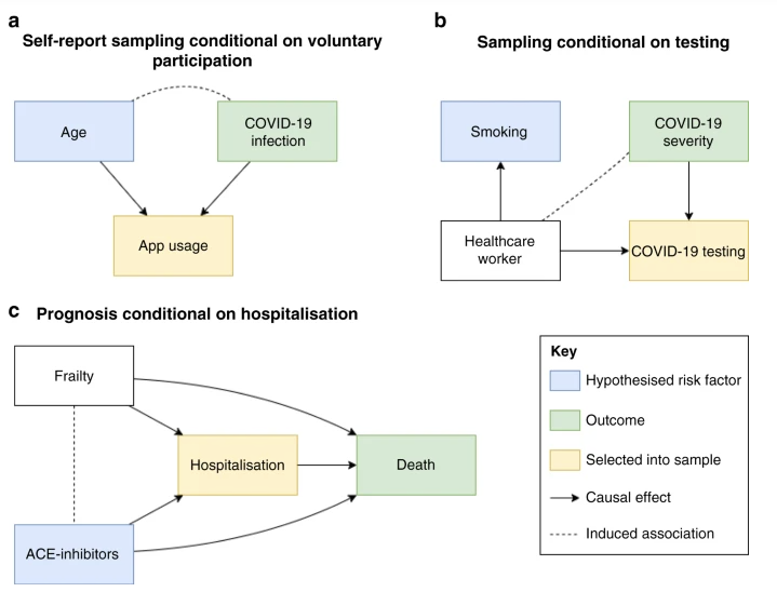
\includegraphics[width=10cm]{select_covid}
	
\end{frame}
%\begin{frame}
%\frametitle{Even more possibilities: reverse causation}
%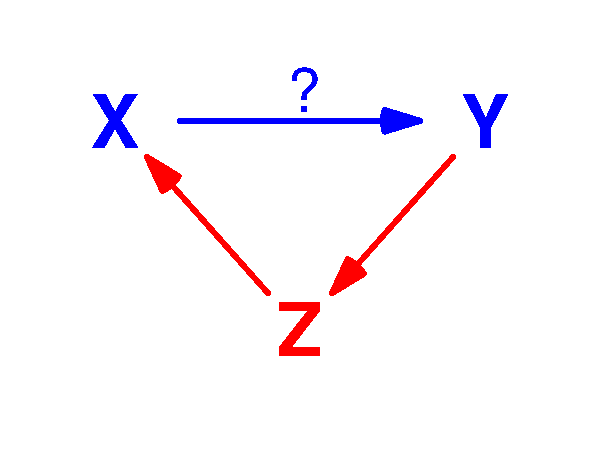
\includegraphics[width=4cm]{revcaus}\\[-0.3cm]

%Now the graph is not any more acyclic -- it is not a DAG!  Can occur by omitting a temporal component. 
%One should modify the graph (and data collection procedure) to enable valid causal inference.     

%\end{frame}


\begin{frame}
 Actually there might be a complicated system of
causal effects:

{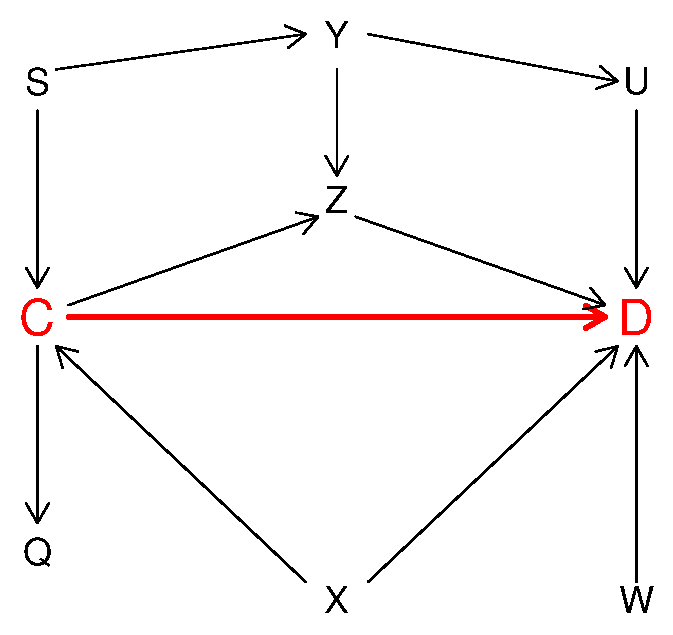
\includegraphics[width=0.4\textwidth]{keeruline2}}\\
{\small  C-smoking; D-cancer \\
Q, S, U, W, X, Y, Z - other factors that influence cancer risks
and/or smoking (genes, social background, nutrition, environment,
personality, \ldots)}
\end{frame}

\begin{frame}
\frametitle{What to do in complicated cases?}

\begin{enumerate}
\item Sketch a causal graph
\item Identify all paths between the exposure and outcome (ways to go from $X$ to $Y$ regardless of the direction of the arrows).
\item Identify the \sini{closed} paths that include colliders and \sini{open} paths that don't.  
\item You need to select adjustment variables that block all \sini{open} paths.
\item \alert{Don't} adjust for colliders (as they would open the closed paths)!
 \item If you are looking for the total effects, you don't need to block the \sini{directed} paths (that follow the directions of the arrows). 
\item \alert{Often, there are unobserved confounders!} 
\end{enumerate}
\mbox{}\\[0.5cm]
R package \textit{dagitty} is useful for such tasks.
\end{frame}


\begin{frame}
\frametitle{Example: mediation with confounding}
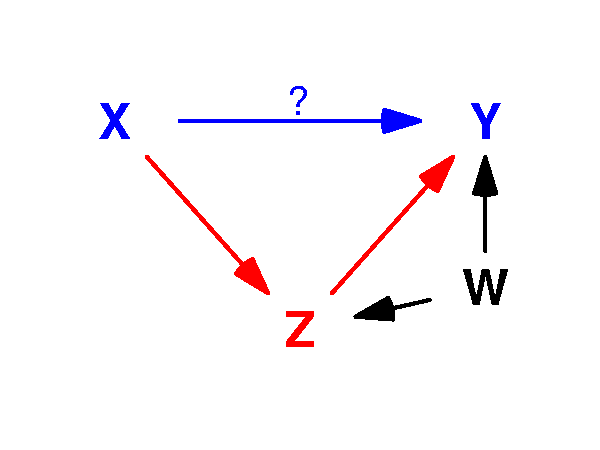
\includegraphics[width=6cm]{mediation_conf}\\[-0.3cm]
Paths:
$X \rightarrow Z \rightarrow Y$ (open) and $X \rightarrow Z \leftarrow W \rightarrow Y$ (closed). \\[0.3cm]
\begin{itemize}
	\item The total effect of $X$ on $Y$ is estimable without any adjustment.
	\item For direct effect you need to adjust for $Z$, but that would open the closed path -- to block that, you also need to adjust for $W$. 
	\item If $W$ is an unobserved confounder, direct effect of $X$ on $Y$ cannot be estimated. 
\end{itemize} 
 
\end{frame}

\section{Causal models for observational data}
\subsection{Instrumental variables estimation}

\begin{frame}
 \frametitle{Instrumental variables estimation: the idea}
A DAG with the exposure $X$, outcome $Y$, confounder $U$ and an \textcolor{blue}{instrument} $Z$:\\[0.2cm]
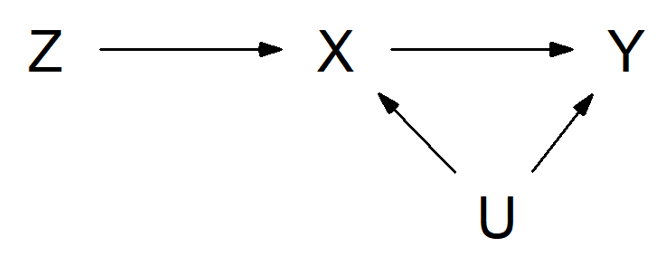
\includegraphics[width=6cm]{IV} \\[0.2cm]
Assuming: \\
$Y= \alpha_y + \beta X + \gamma U +\epsilon,  \  \E(\epsilon|X,U)=0$, \\[0.2cm]
simple regression will estimate: \\[0.2cm]
$\E(Y|X)= \alpha_y + \beta X + \gamma \E(U|X)$. \\[0.3cm]
\alert{Thus the coefficient of $X$ will be a biased estimate of $\beta$ (as it also depends on $\gamma$). }
\end{frame}

\begin{frame}
	\frametitle{Instrumental variables estimation: the idea}
	\begin{columns}
		\begin{column}{7cm}
\mbox{}\\
			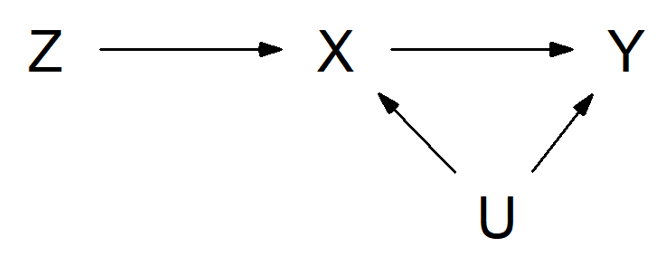
\includegraphics[width=6cm]{IV} \\[0.5cm]
		\begin{block}{}
		A variable $Z$ is an  \textcolor{blue}{instrument} for the path $X \rightarrow Y$, if: \begin{enumerate}
			\item $Z$ has a direct causal effect on $X$
			\item $Z$ does not have any direct or indirect causal effect on $Y$ or the confounders $U$.
		\end{enumerate}
	\end{block}
			\end{column}
		\begin{column}{6cm}
			\begin{block}{}
				\begin{itemize}
					\item 
				It can be shown that the causal effect of $X$ on $Y$ equals:
				$$
				\beta = \frac{cov(Z,Y)}{cov(Z,X)} =  \frac{\beta_{ZY}}{\beta_{ZX}},
				$$
				where $\beta_{ZY}$ and $\beta_{ZX}$ are the coefficients of $Z$ in a simple linear regression models for  $Y$ and $X$ (with covariate $Z$).
\item Replacing $\beta_{ZY}$ and $\beta_{ZX}$ by their estimates, we get the  \alert{instrumental variables (IV) estimate} of $\beta$. 
				\end{itemize}
				
				
			\end{block}
		\end{column}
	\end{columns}
\end{frame}



\begin{frame}
			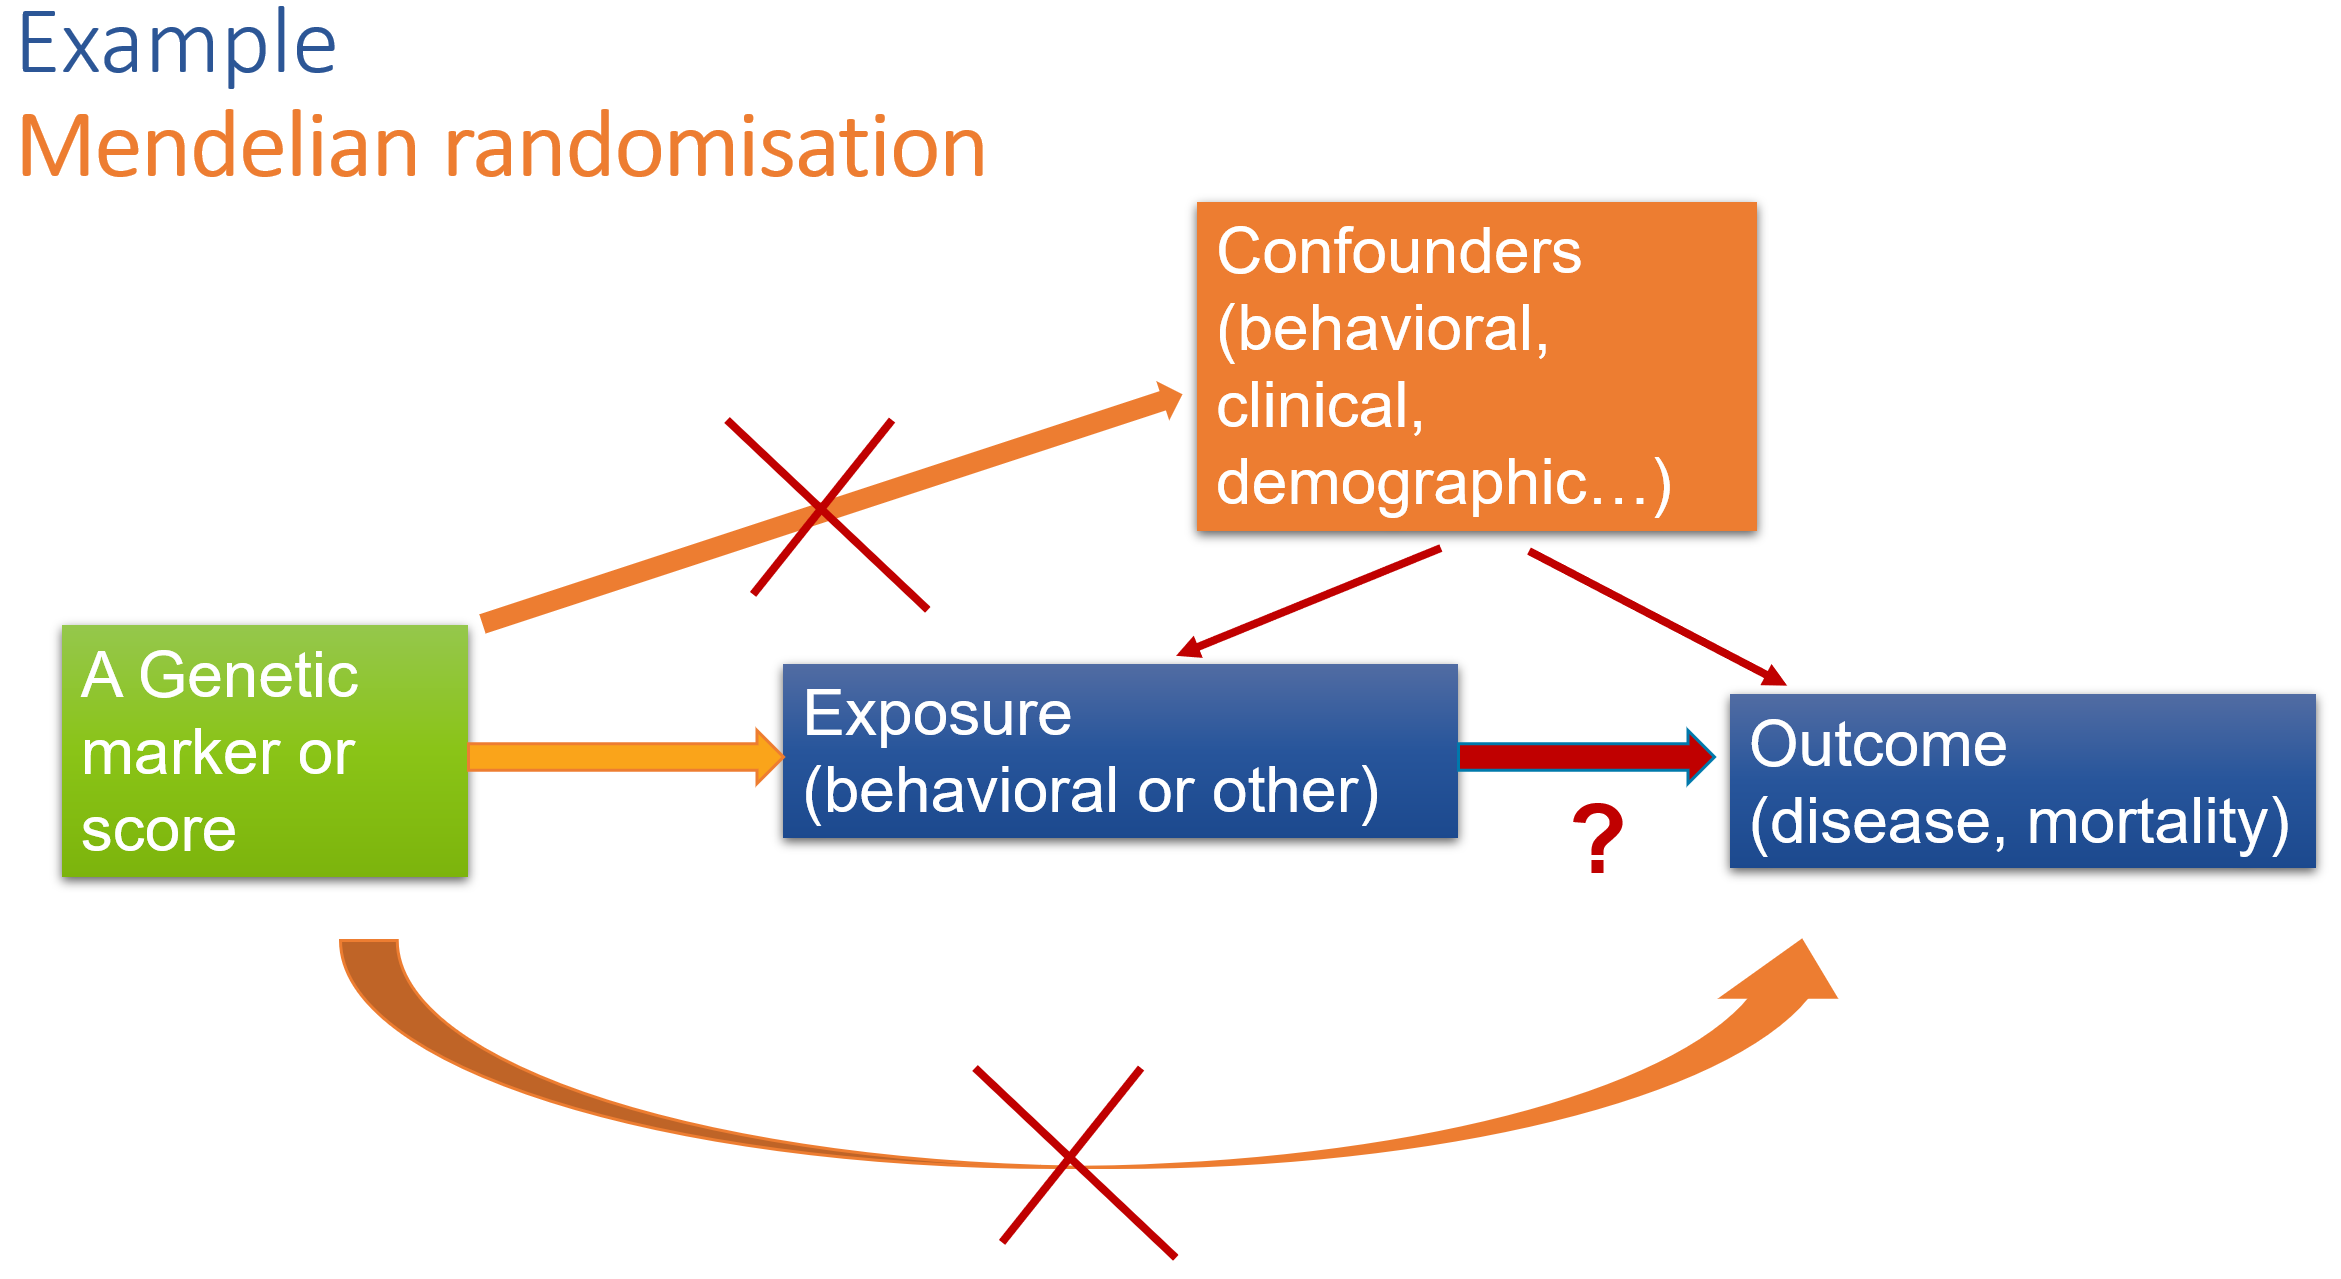
\includegraphics[width=12cm]{MR_varviline} 
		\end{frame}


\section{Summary and references}
\begin{frame}
\frametitle{Summary}
\begin{itemize}
\item There is no unique definition of ``the causal effect'' 
\item The validity of any causal effect estimates depends on the validity of the underlying assumptions.
\item Adjustment for other available variables may remove (some) confounding, but it may also create more confounding. \alert{Do not adjust for variables that may themselves be affected by the outcome.}   
\item Instrumental variables approaches can be helpful, but beware of assumptions! 
\end{itemize}
\end{frame}



\begin{frame}
\setlength{\textwidth}{1.2\textwidth}
\frametitle{Some references}
\begin{itemize}
\item A webpage and a free online book by Miguel Hernan and Jamie Robins: 
\href{http://www.hsph.harvard.edu/miguel-hernan/causal-inference-book/}{http://www.hsph.harvard.edu/miguel-hernan/causal-inference-book/}
\item Judea Pearl, ``The Book of Why'' 
\item Mendelian randomization:  
Sheehan, N., Didelez, V., et al., Mendelian Randomization and Causal Inference in Observational Epidemiology, PLoS Med. 2008; papers by G.D. Smith, J. Bowden, S. Burgess and others.  
%\item \textit{An overview of Mendelian randomization}: 
\end{itemize}

\includegraphics[width=3cm]{whatif}

\includegraphics[width=2.5cm]{why}
\end{frame}
\end{document}

